\section{学习信念表征}

本节介绍针对常值延迟学习信念表征的方法。
学习完成后，该表征可作为状态的替代与任何\gls{rl}算法配合使用。
随后通过一个简单技巧将该方法扩展为同时学习多个延迟。

\subsection{信念表征网络}
\label{subsec:belief_net}

为了对某个增广状态 $x=(s,a_1,\dots,a_{\delay})\in\augmentedstate$ 学习信念 $\augmentedbelief(\cdot\vert x)$，需要预测增广状态中包含的动作的影响。
一种方法是用循环函数近似转移动力学。
循环\gls{nn}可作为近似器，但此类网络训练和评估速度较慢。
本文改用参数为 $\vectorialform{\phi}$ 的\gls{nn} $f_{\vectorialform{\phi}}$ 直接处理整个输入，要求网络一次性输出所有未观测状态的信念表征。
该网络有多种方式处理增广状态。
本文选择从增广状态构造序列 $(s,a_{i})_{i \in [\![1,\delay]\!]}$。
该序列随后输入因果 Transformer（causal Transformer）~\cite{vaswani2017attention}的编码器网络（见~\Cref{subsubsec:transformer}），记为 $f_{\vectorialform{\phi}}$。
选择因果 Transformer 主要基于三个原因：Transformer 在序列到序列任务中取得优异实证结果\cite{devlin2018bert}；可使用掩码保持因果性，这对过去信念不依赖未来信念的特性很有用；Transformer 中的位置编码可添加动作在序列中位置的信息，因此同一动作在增广状态中不同位置可产生不同影响。

为训练 $f_{\vectorialform{\phi}}$ 有效编码信念，本文使用\gls{maf}~\cite{papamakarios2017masked}网络（见~\Cref{subsubsec:maf}）。
选择基于其近似概率分布的能力。
该网络记为 $f_{\vectorialform{\theta}}$，将 $f_{\vectorialform{\phi}}$ 的输出作为其概率的条件。
然后，该网络接受训练，仅从 $f_{\vectorialform{\phi}}$ 给出的条件近似未观测状态的概率。
通过这种方式，所有关于信念的信息都将编码于 $f_{\vectorialform{\phi}}$ 中。
注意，\gls{maf}网络的损失梯度可通过其条件传播，因此可同时用于训练 $f_{\vectorialform{\phi}}$。

下面更精确地考察信念网络内部的工作机制。
设 $x=(s,a_1,\dots,a_{\delay})$ 为当前增广状态。首先，Transformer 为 $(s,a_{i})_{i \in [\![1,\delay]\!]}$ 中的每个元素 $(s,a_{i})$ 输出一个向量 $f_{\vectorialform{\phi}}(x)_i\in\realnumbers^{n_b}$。
记 $n_b$ 为信念表征的维度。
设 $(s_1,\dots,s_{\delay})$ 为将要近似信念的 $\delay$ 个未观测状态，$\augmentedbelief[i](\cdot\vert x)$ 为 $s_i$ 的信念。
如 \Cref{subsubsec:maf} 所述，\gls{maf}递归地将参数化函数应用于基础密度 $p_u$，将其变换为密度 $p_{\theta}$。
基础密度 $p_u$ 采用正态分布。
与传统设定的不同之处在于，此处相对于 \Cref{eq:p_inverted_maf} 增加了对 $f_{\vectorialform{\phi}}({x})_i$ 的条件化。
\begin{align*}
    p_{\vectorialform{\theta}}(s_i\vert f_{\vectorialform{\phi}}({x})_i) = p_u(f_\theta^{-1}(s_i,f_{\vectorialform{\phi}}({x})_i)) \left\lvert \det\left(\frac{\partial f_\theta^{-1}}{\partial s_i}\right)\right\rvert.
\end{align*}
注意，MAF 的构建模块 MADE 层（见~\Cref{subsubsec:maf}）只需一次前向传播即可计算密度，而采样则需要与输出维度相同次数的前向传播。
这一点在此处不构成限制，因为本文不需要从信念中采样状态，只需学习其近似。

然后训练\gls{maf}最小化其密度与训练集密度之间的 Kullback-Leibler 散度。
此处损失函数为
\begin{align*}
    \min_{\vectorialform{\theta},\vectorialform{\phi}} \sum_{i=1}^\delay \kullbackleiblerdivergence( \augmentedbelief[i](s_i \vert  x) \Vert p_{\vectorialform{\theta}}(s_i\vert f_{\vectorialform{\phi}}({x})_i)).
\end{align*}
该量天然可微，可通过基于梯度的优化方法最小化。
对于 $N$ 个增广状态的样本 $(x^k)_{1\le k\le N}$，其中 $x^k=(s^k,a^k_1,\dots,a^k_{\delay})$，损失函数可近似为
\begin{align}
\label{eq:loss_maf}
    \mathcal{L}_p = \sum_{k=1}^N \sum_{i=1}^\delay \log p_{\vectorialform{\theta}}(s^{k}_{i}\vert f_{\vectorialform{\phi}}(x^k)_i).
\end{align}
信念表征网络的图形表示见\Cref{fig:dtrpo_network}，其训练过程见\Cref{algo:belief_training}。
在\gls{rl}中，通常使用回放缓冲区补偿因训练而随时间演化的采样策略。
这也使框架更接近监督学习。
本文采用相同思路，将增广状态保存在回放缓冲区中。

信念表征网络可作为状态的预处理与任何\gls{rl}算法配合使用。
在实验部分，本文将该网络接入\gls{trpo} \cite{schulman2015trust}，并将该方法称为 Delayed-TRPO (D-TRPO)。

\begin{figure}[t]
    \centering
    \resizebox{10cm}{!}{%
    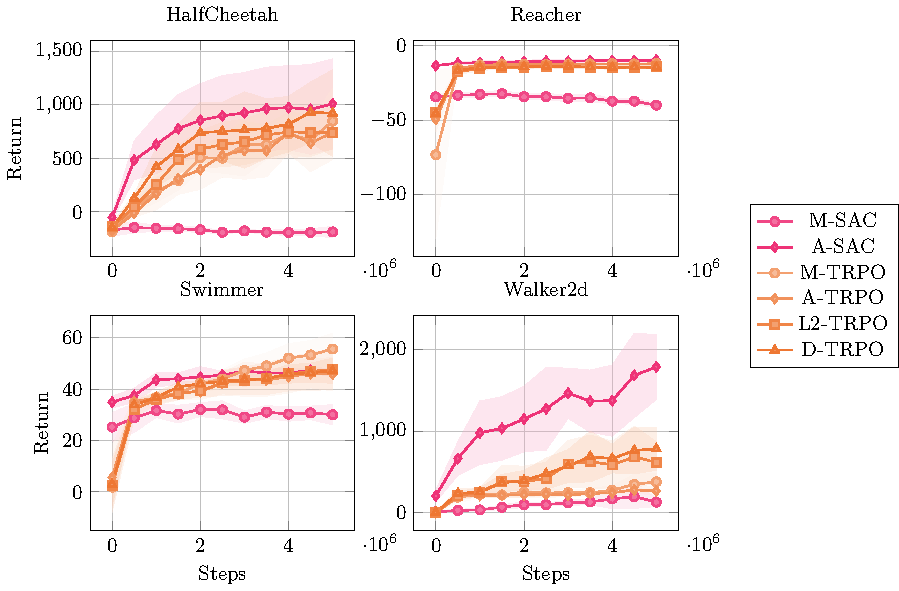
\includegraphics[labelbelief=dtrponetwork]{img/thesis_plots_belief.pdf}
    }
    \caption{D-TRPO 网络。从下至上：增广状态被拆分为序列 $(s,a_{i})_{i \in [\![1,\delay]\!]}$；序列经过一个 Transformer 编码器层，返回信念编码 $f_{\vectorialform{\phi}}(x)_i\in\realnumbers^{n_b}$；MAF 层以前一个编码向量为条件学习后续 $\delay$ 个状态的信念。最后，最后一个信念编码 $f_{\vectorialform{\phi}}(x)_\delay$ 用作策略的输入。}
    \label{fig:dtrpo_network}
\end{figure}


\begin{algorithm}[t]
\caption{信念表征网络训练}\label{algo:belief_training}
\textbf{Inputs}:
belief representation network parameters $\vectorialform{\phi}$ and $\vectorialform{\theta}$, number of epochs $K$, batch size $N$,number of samples $M$, empty replay buffer $\mathcal{D}$.\\
\textbf{Outputs}: Trained parameters $\vectorialform{\phi}$ and $\vectorialform{\theta}$.
\begin{algorithmic}[1]
    \FOR{$k=1,\dots,K$}%\{$1,\dots,N$\}}
        \STATE Collect $M$ samples under some policy $\pi$
        \STATE Add couples of augmented states $x=(s,a_1,\dots,a_{\delay})$ and corresponding sequence states to be predicted $(s_1,\dots,s_\delay)$ to $\mathcal{D}$
        \STATE Sample $N$ such couples from $\mathcal{D}$
        \STATE Update parameters $\vectorialform{\phi}$ and $\vectorialform{\theta}$ by descending the gradient $\nabla_{\vectorialform{\phi},\vectorialform{\theta}}\mathcal{L}_p$ (See \Cref{eq:loss_maf})
    \ENDFOR
\end{algorithmic}
\end{algorithm}

\subsection{同时学习多个延迟}
\label{subsec:multi_delay_once_belief}
本文提出一个简单思路，利用 D-TRPO 在给定整数延迟 $\delay>0$ 下学习的策略。
尽管思路简单，但先前文献未曾考虑过此想法。
本文提出通过模拟 $\delay$ 延迟，将 D-TRPO 应用于更小的整数延迟 $0<\delay'<\delay$。
具体而言，除了延迟 $\delay'$ 对应的增广状态 $x_t=(s_{t-\delay'},a_{t-\delay'},\dots,a_{t-1})$ 外，还考虑一个缓冲区，
\begin{align*}
    (s_{t-\delay},a_{t-\delay},\dots,s_{t-\delay'-1},a_{t-\delay'-1}),
\end{align*}
包含 $t-\delay'$ 之前最后 $\delay-\delay'$ 个状态和动作的历史记录。
通过这种方式，智能体可以构造一个合成增广状态 $x_t'=(s_{t-\delay},a_{t-\delay},\dots,a_{t-1})$。
这足以应用 D-TRPO 在延迟 $\delay$ 下学习的策略。
显然，该算法具有与延迟 $\delay$ 的 D-TRPO 相同的性能保证。
在\Cref{sec:exp_belief}中提供实验验证该思路的有效性。

对于文献中的某些方法，可以做得比上述简单思路更好。
例如，与\cite{firoiu2018human}类似，可以不学习信念表征，而是学习未来所有 $\delay$ 个状态的期望状态。
本文设计一种方法实现这一目标，使用与 D-TRPO 相同的网络结构，但移除 MAF 层。
网络训练以最小化其输出 $(f_\phi(\textbf{x})_i)_{i\in[\![1, d]\!]}$ 与真实状态 $(s_1,\dots,s_\delay)$ 之间的 L2 损失。
将其接入\gls{trpo}后，称该方法为 L2-TRPO。
在这种情况下，可以用另一种方式同时学习多个延迟。
事实上，因果 Transformer 网络的一个有趣特性是它可以被裁剪到所需长度，因此可以应用于更短延迟 $0<\delay'<\delay$ 的增广状态。
根据设计，L2-TRPO 也已学习未来 $\delay'$ 步的期望状态。
因此，裁剪后 Transformer 的输出可作为\gls{trpo}的输入。
值得注意的是，D-TRPO 无法做到这一点。尽管它学习了未来每个 $\delay$ 状态的信念表征，但各自的编码可能遵循不同规则。
因此，\gls{trpo}可能无法理解较早状态的编码。

此处提出的简单思路与\cite{chen2021delay}的论点一致：基于模型的方法更适合延迟场景，因为其模型可以复用。


